% ----------------------------------------------------------
\chapter{Diagrama de Casos de Uso}
\label{apendice:casos_de_uso}
% ----------------------------------------------------------

Este apêndice apresenta o Diagrama de Casos de Uso do sistema \textit{FaunaMar}, um artefato da UML (Unified Modeling Language) que foi central para a definição do escopo do projeto. O diagrama modela as funcionalidades do software sob a perspectiva do usuário, ilustrando de forma gráfica as interações entre os atores e o sistema.

Nele, são identificados os dois atores principais: o Cientista Cidadão, representando o público geral que contribui com os registros, e o Pesquisador, responsável pela validação, gerenciamento e análise dos dados. Os casos de uso, representados por elipses, descrevem as ações disponíveis para cada ator. Este modelo serviu como guia fundamental durante a fase de levantamento de requisitos e orientou o desenvolvimento das funcionalidades descritas no Capítulo \ref{cap:resultados_obtidos}.

\begin{figure}[htb]
    \centering
    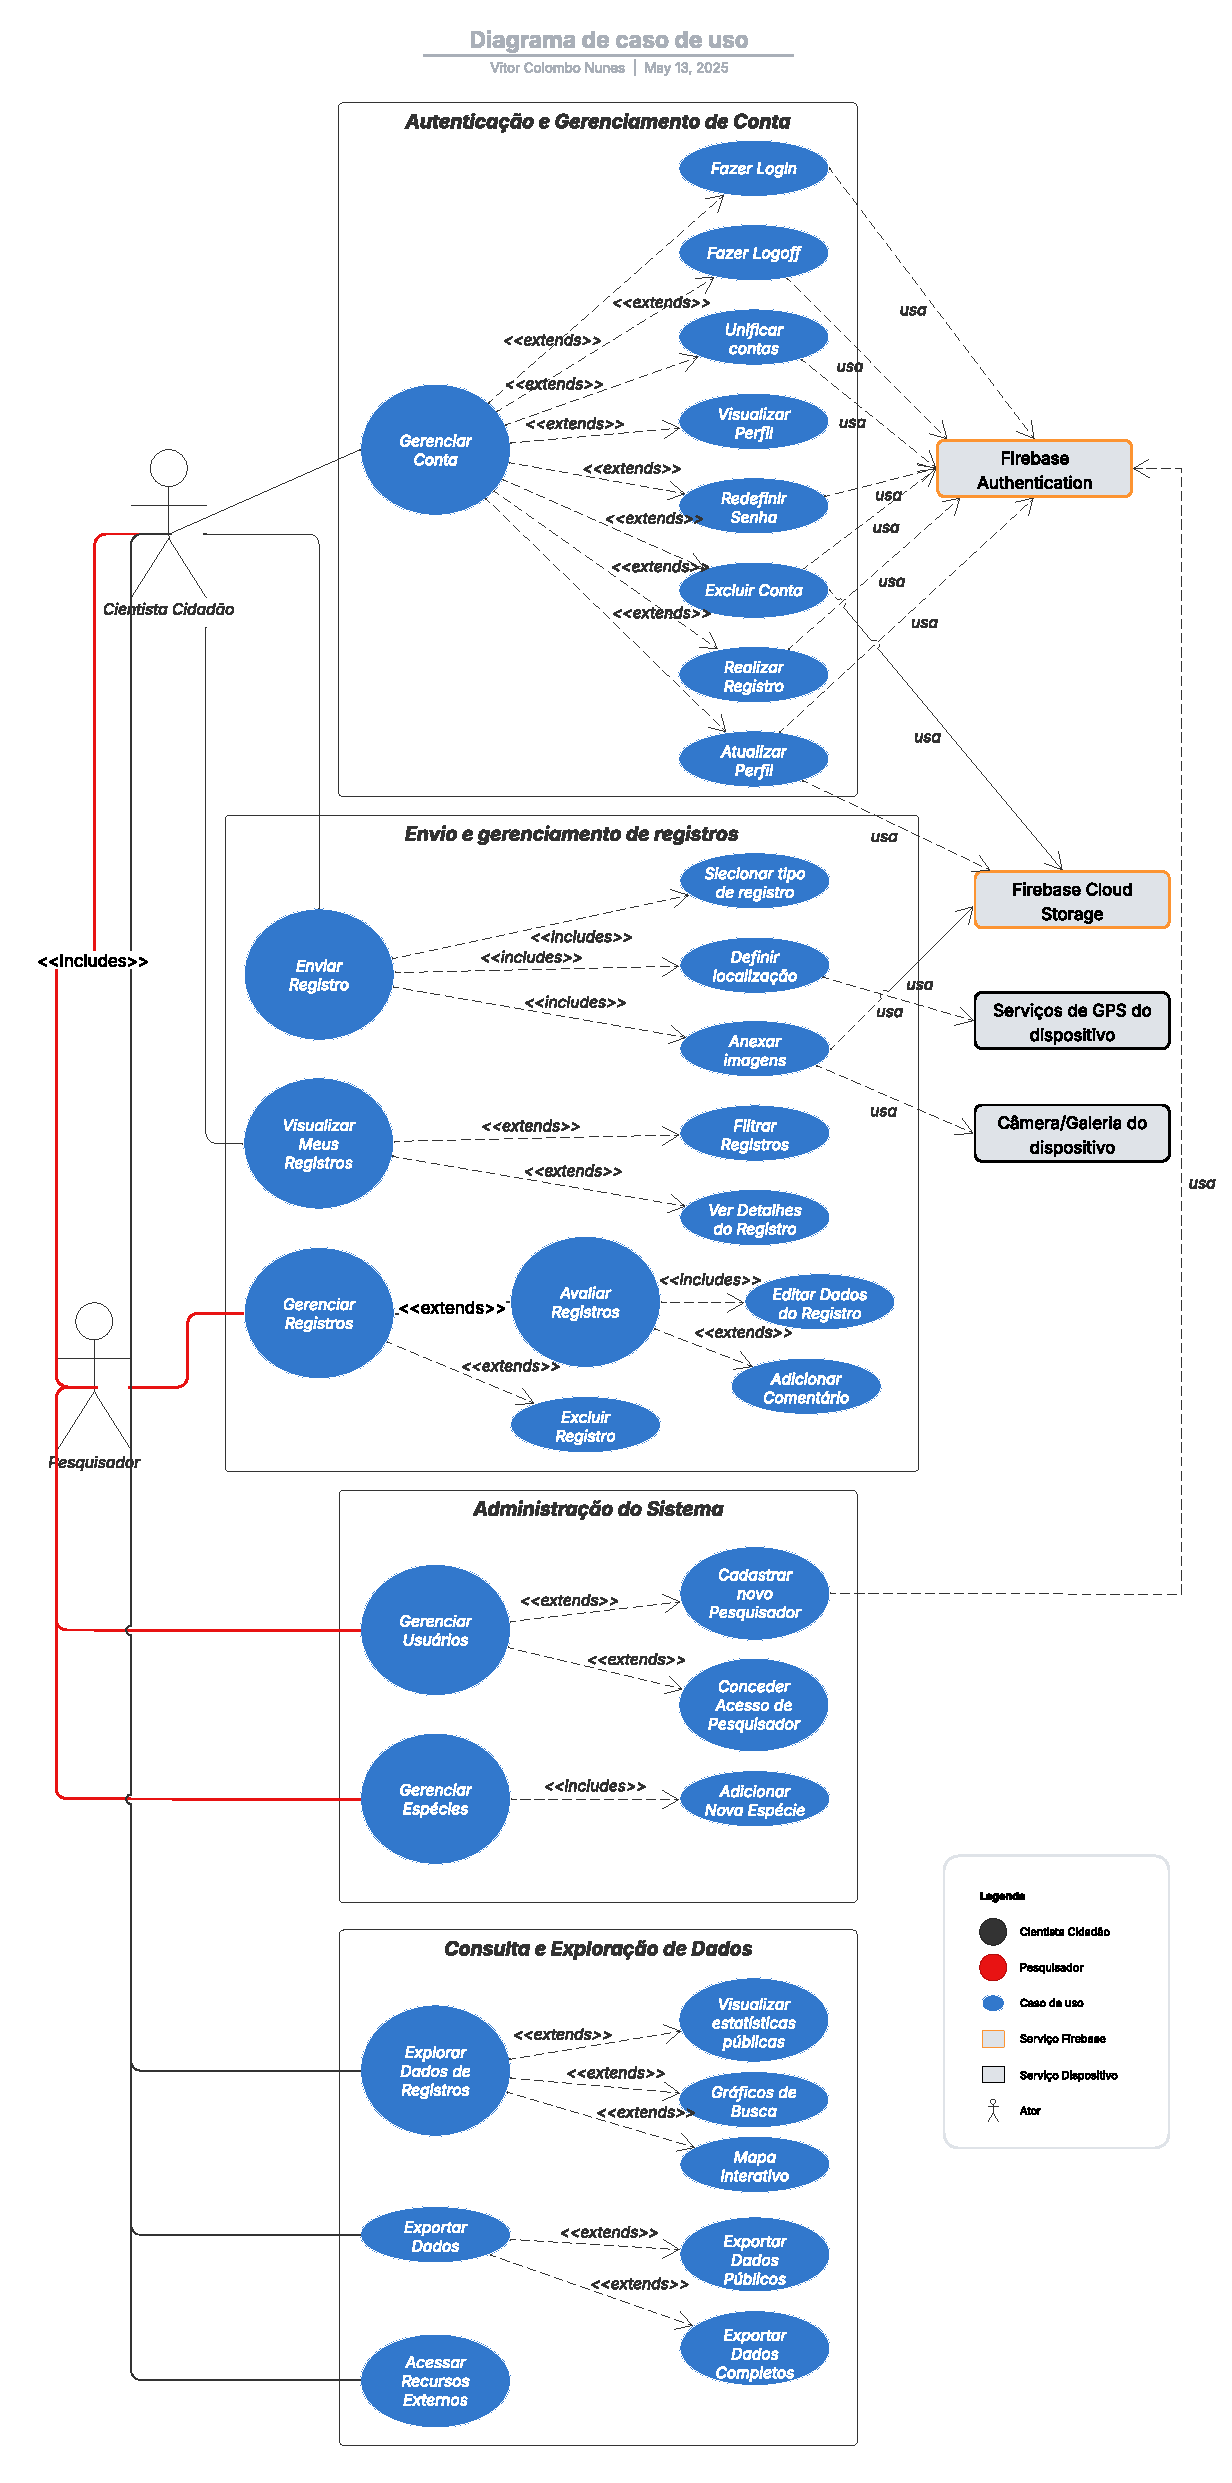
\includegraphics[width=0.8\textwidth]{diagrams/Diagrama de caso de uso (1).pdf}
    \caption{Diagrama de Casos de Uso do sistema \textit{FaunaMar}.}
    \label{fig:diagrama-casos-uso}
    \legend{Fonte: Autor}
\end{figure}